\documentclass[]{article}
\usepackage[left=1in,top=1in,right=1in,bottom=1in]{geometry}


%%%% more monte %%%%
\usepackage{wrapfig}
% thispagestyle{empty}
% https://stackoverflow.com/questions/2166557/how-to-hide-the-page-number-in-latex-on-first-page-of-a-chapter
\usepackage{color}
% \usepackage[table]{xcolor} % are they using color?

% \definecolor{WSU.crimson}{HTML}{981e32}
% \definecolor{WSU.gray}{HTML}{5e6a71}

% \definecolor{shadecolor}{RGB}{248,248,248}
\definecolor{WSU.crimson}{RGB}{152,30,50} % use http://colors.mshaffer.com to convert from 981e32
\definecolor{WSU.gray}{RGB}{94,106,113}

%%%%%%%%%%%%%%%%%%%%%%%%%%%%

\newcommand*{\authorfont}{\fontfamily{phv}\selectfont}
\usepackage{lmodern}


  \usepackage[T1]{fontenc}
  \usepackage[utf8]{inputenc}




\usepackage{abstract}
\renewcommand{\abstractname}{}    % clear the title
\renewcommand{\absnamepos}{empty} % originally center

\renewenvironment{abstract}
 {{%
    \setlength{\leftmargin}{0mm}
    \setlength{\rightmargin}{\leftmargin}%
  }%
  \relax}
 {\endlist}

\makeatletter
\def\@maketitle{%
  \pagestyle{empty}
  \newpage
%  \null
%  \vskip 2em%
%  \begin{center}%
  \let \footnote \thanks
    {\fontsize{18}{20}\selectfont\raggedright  \setlength{\parindent}{0pt} \@title \par}%
}
%\fi
\makeatother









\title{\textbf{\textcolor{WSU.crimson}{Will Is Better than
Denzel}} \newline \textbf{\textcolor{WSU.gray}{An Analysis of the Career
of Will Smith vs Denzel Washington}}  }
 

%  

% \author{ \Large true \hfill \normalsize \emph{} }
\author{\Large Peyton
Urquhart\vspace{0.05in} \newline\normalsize\emph{Student of Software
Engineering (WSU)}  }


\date{April 11, 2021}
\setcounter{secnumdepth}{3}

\usepackage{titlesec}
% See the link above: KOMA classes are not compatible with titlesec any more. Sorry.
% https://github.com/jbezos/titlesec/issues/11
\titleformat*{\section}{\bfseries}
\titleformat*{\subsection}{\bfseries\itshape}
\titleformat*{\subsubsection}{\itshape}
\titleformat*{\paragraph}{\itshape}
\titleformat*{\subparagraph}{\itshape}

% https://code.usgs.gov/usgs/norock/irvine_k/ip-092225/


%\titleformat*{\section}{\normalsize\bfseries}
%\titleformat*{\subsection}{\normalsize\itshape}
%\titleformat*{\subsubsection}{\normalsize\itshape}
%\titleformat*{\paragraph}{\normalsize\itshape}
%\titleformat*{\subparagraph}{\normalsize\itshape}

% https://tex.stackexchange.com/questions/233866/one-column-multicol-environment#233904
\usepackage{environ}
\NewEnviron{auxmulticols}[1]{%
  \ifnum#1<2\relax% Fewer than 2 columns
    %\vspace{-\baselineskip}% Possible vertical correction
    \BODY
  \else% More than 1 column
    \begin{multicols}{#1}
      \BODY
    \end{multicols}%
  \fi
}





\usepackage{natbib}
\setcitestyle{aysep={}} %% no year, comma just year
% \usepackage[numbers]{natbib}
\bibliographystyle{./../../latex-setup/biblio/ormsv080.bst}



\usepackage[strings]{underscore} % protect underscores in most circumstances




\newtheorem{hypothesis}{Hypothesis}
\usepackage{setspace}


%%%%%%%%%%%%%%%%%%%%%%%%%%%%%%%%%%%%%%%%%%%%%%%%%%%%%
%%% MONTE ADDS %%%

\usepackage{fancyhdr} % fancy header 
\usepackage{lastpage} % last page 

\usepackage{multicol}


\usepackage{etoolbox}
\AtBeginEnvironment{quote}{\singlespacing\small}
% https://tex.stackexchange.com/questions/325695/how-to-style-blockquote


\usepackage{soul}			%% allows strike-through
\usepackage{url}			%% fixes underscores in urls
\usepackage{csquotes}		%% allows \textquote in references
\usepackage{rotating}		%% allows table and box rotation
\usepackage{caption}		%% customize caption information
\usepackage{booktabs}		%% enhance table/tabular environment
\usepackage{tabularx}		%% width attributes updates tabular
\usepackage{enumerate}		%% special item environment
\usepackage{enumitem}		%% special item environment

\usepackage{lineno}		%% allows linenumbers for editing using \linenumbers
\usepackage{hanging}


\usepackage{mathtools}  	%% also loads amsmath
\usepackage{bm}		%% bold-math
\usepackage{scalerel}	%% scale one element (make one beta bigger font)

\newcommand{\gFrac}[2]{ \genfrac{}{}{0pt}{1}{{#1}}{#2} }

\newcommand{\betaSH}[3]{  \gFrac{\text{\tiny #1}}{{\text{\tiny #2}}}\hat{\beta}_{\text{#3}}   }
\newcommand{\betaSB}[3]{              ^{\text{#1}} _{\text{#2}} \bm{\beta} _{\text{#3}}                   }  %% bold
\newcommand{\bigEQ}{  \scaleobj{1.5}{{\ }= } }
\newcommand{\bigP}[1]{  \scaleobj{1.5}{#1 } }





\usepackage{endnotes}  % he already does this ...
\renewcommand{\enotesize}{\normalsize}
% https://tex.stackexchange.com/questions/99984/endnotes-do-not-be-superscript-and-add-a-space
\renewcommand\makeenmark{\textsuperscript{[\theenmark]}} % in brackets %
% https://tex.stackexchange.com/questions/31574/how-to-control-the-indent-in-endnotes
\patchcmd{\enoteformat}{1.8em}{0pt}{}{}

\patchcmd{\theendnotes}
  {\makeatletter}
  {\makeatletter\renewcommand\makeenmark{\textbf{[\theenmark]} }}
  {}{}



% https://tex.stackexchange.com/questions/141906/configuring-footnote-position-and-spacing

\addtolength{\footnotesep}{5mm} % change to 1mm

\renewcommand{\thefootnote}{\textbf{\arabic{footnote}}}
\let\footnote=\endnote
%\renewcommand*{\theendnote}{\alph{endnote}}
%\renewcommand{\theendnote}{\textbf{\arabic{endnote}}}


\renewcommand*{\notesname}{}

\makeatletter
\def\enoteheading{\section*{\notesname
  \@mkboth{\MakeUppercase{\notesname}}{\MakeUppercase{\notesname}}}%
  \mbox{}\par\vskip-2.3\baselineskip\noindent\rule{.5\textwidth}{0.4pt}\par\vskip\baselineskip}
\makeatother


\renewcommand*{\contentsname}{}

\renewcommand*{\refname}{REFERENCES}


%\usepackage{subfigure}
\usepackage{subcaption}

\captionsetup{labelfont=bf}  % Make Table / Figure bold

%%% you could add elements here ... monte says .... %%%
%\usepackage{mypackageForCapitalH}


%%%%%%%%%%%%%%%%%%%%%%%%%%%%%%%%%%%%%%%%%%%%%%%%%%%%%

% set default figure placement to htbp
\makeatletter
\def\fps@figure{htbp}
\makeatother


% move the hyperref stuff down here, after header-includes, to allow for - \usepackage{hyperref}

\makeatletter
\@ifpackageloaded{hyperref}{}{%
\ifxetex
  \PassOptionsToPackage{hyphens}{url}\usepackage[setpagesize=false, % page size defined by xetex
              unicode=false, % unicode breaks when used with xetex
              xetex]{hyperref}
\else
  \PassOptionsToPackage{hyphens}{url}\usepackage[draft,unicode=true]{hyperref}
\fi
}

\@ifpackageloaded{color}{
    \PassOptionsToPackage{usenames,dvipsnames}{color}
}{%
    \usepackage[usenames,dvipsnames]{color}
}
\makeatother
\hypersetup{breaklinks=true,
            bookmarks=true,
            pdfauthor={Peyton Urquhart (Student of Software Engineering
(WSU))},
             pdfkeywords = {data analytics; data science;},  
            pdftitle={Will Is Better than Denzel: An Analysis of the
Career of Will Smith vs Denzel Washington},
            colorlinks=true,
            citecolor=blue,
            urlcolor=blue,
            linkcolor=magenta,
            pdfborder={0 0 0}}
\urlstyle{same}  % don't use monospace font for urls

% Add an option for endnotes. -----

%
% add tightlist ----------
\providecommand{\tightlist}{%
\setlength{\itemsep}{0pt}\setlength{\parskip}{0pt}}

% add some other packages ----------

% \usepackage{multicol}
% This should regulate where figures float
% See: https://tex.stackexchange.com/questions/2275/keeping-tables-figures-close-to-where-they-are-mentioned
\usepackage[section]{placeins}



\pagestyle{fancy}   
\lhead{\textcolor{WSU.crimson}{\textbf{ Will Is Better than Denzel }}}
\chead{}
\rhead{\textcolor{WSU.gray}{\textbf{  Page\ \thepage\ of\ \protect\pageref{LastPage} }}}
\lfoot{}
\cfoot{}
\rfoot{}


\begin{document}
	
% \pagenumbering{arabic}% resets `page` counter to 1 
%    

% \maketitle

{% \usefont{T1}{pnc}{m}{n}
\setlength{\parindent}{0pt}
\thispagestyle{plain}
{\fontsize{18}{20}\selectfont\raggedright 
\maketitle  % title \par  

}

{
   \vskip 13.5pt\relax \normalsize\fontsize{11}{12} 
   
\textbf{\authorfont Peyton Urquhart} \hskip 15pt \emph{\small Student of
Software Engineering (WSU)}   

}

}








\begin{abstract}

    \hbox{\vrule height .2pt width 39.14pc}

    \vskip 8.5pt % \small 

\noindent Data from IMDB is analyzed for actors Will Smith and Denzel
Washington. This report aims to portray Will Smith as a better actor
than Denzel Washginton. The approach I found best was to contrast the
financial and popular careers of the actors (rather than critic/audience
ratings).


\vskip 8.5pt \noindent \textbf{\underline{Keywords}:} data analytics;
data science; \par

    




    
    \hbox{\vrule height .2pt width 39.14pc}
    \vskip 5pt 
    \hfill \textbf{\textcolor{WSU.gray}{ April 11, 2021 } }
    \vskip 5pt 
    
\end{abstract}


\vskip -8.5pt



 % removetitleabstract

\noindent  

\begin{figure}[!ht]
 \label{fig:one-graphic}
%% figures have hrule, tables have hline
    \begin{center}
        \scalebox{1.00}{    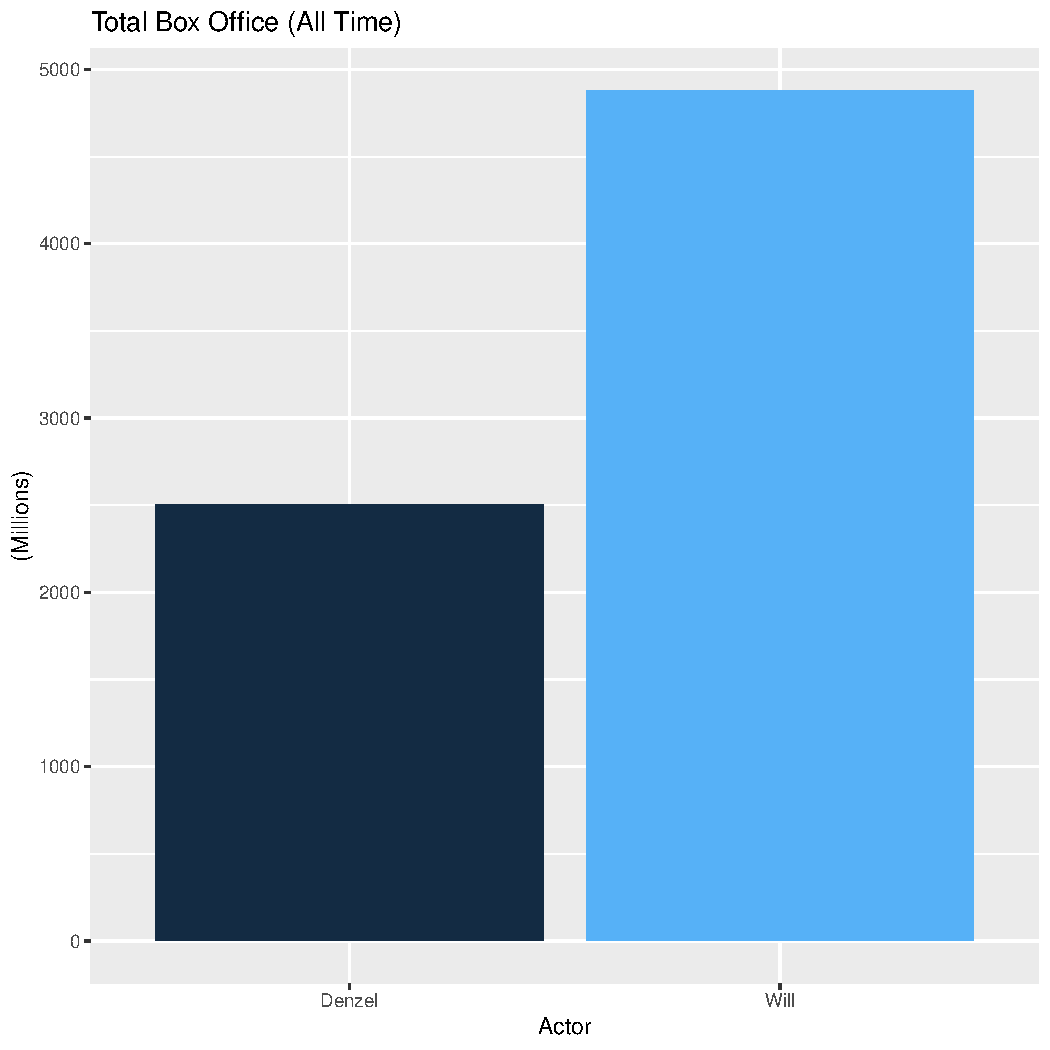
\includegraphics{figures/Total-Box.pdf} }
    \end{center}
    \hrule
      \vspace{2mm}
    \caption{ \textbf{All-Time Box Office Sales for Will and Denzel:} \newline \footnotesize{ Box-office revenue
    for Will Smith's 60 most popular movies capture the vast majority of Sales in his career.\newline \newline
    Approaching 5-billion, Will has accomplished approximately twice the revenue as Denzel washington in 
    about 10 less years in the industry. }  }
    \vspace{2mm}
    \hrule
\end{figure}

\begin{figure}[!ht]
 \label{fig:one-graphic}
%% figures have hrule, tables have hline
    \begin{center}
        \scalebox{1.00}{    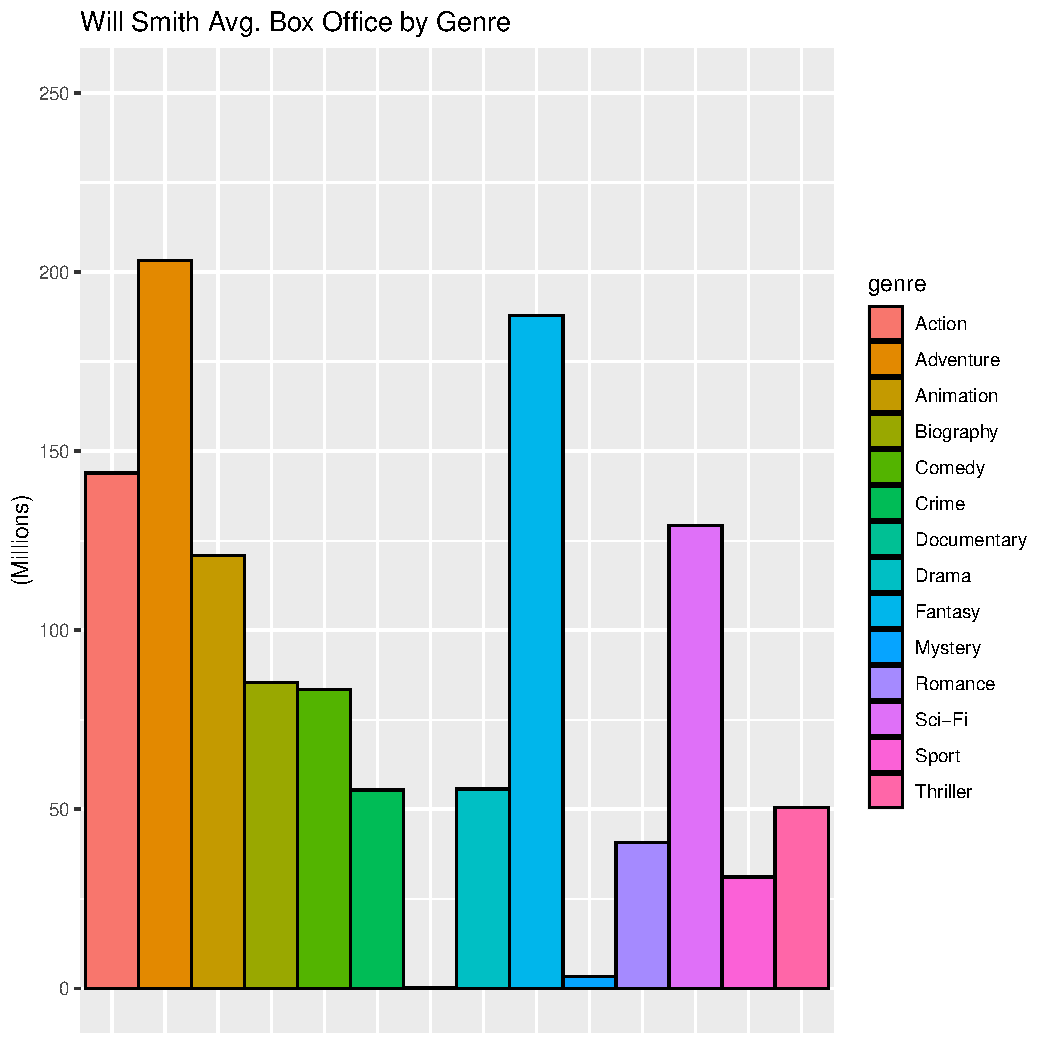
\includegraphics{figures/Will-Box-By-Genre.pdf} }
    \end{center}
    \hrule
      \vspace{2mm}
    \caption{ \textbf{Will Smith Box Office Revenue by Genre:} \newline \footnotesize{ Average box
    office sales for each of Will Smith's movies tagged with a particular Genre on IMDB}  }
    \vspace{2mm}
    \hrule
\end{figure}

\begin{figure}[!ht]
 \label{fig:one-graphic}
%% figures have hrule, tables have hline
    \begin{center}
        \scalebox{1.00}{    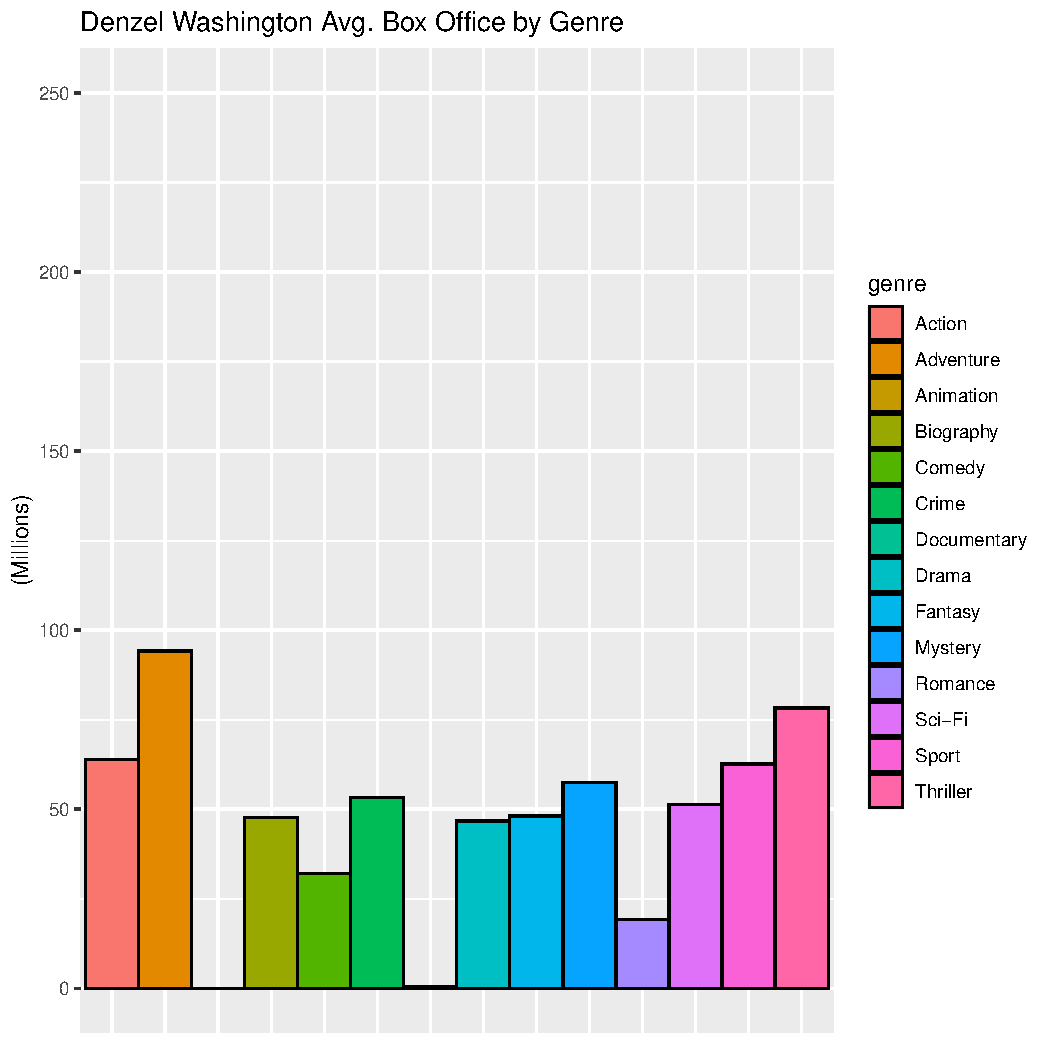
\includegraphics{figures/Denz-Box-By-Genre.pdf} }
    \end{center}
    \hrule
      \vspace{2mm}
    \caption{ \textbf{Denzel Washington Box Office Revenue by Genre:} \newline \footnotesize{ Average box
    office sales for each of Denzels's movies tagged with a particular Genre on IMDB}  }
    \vspace{2mm}
    \hrule
\end{figure}

\begin{figure}[!ht]
 \label{fig:one-graphic}
%% figures have hrule, tables have hline
    \begin{center}
        \scalebox{1.00}{    \includegraphics{figures/Avg-votes.pdf} }
    \end{center}
    \hrule
      \vspace{2mm}
    \caption{ \textbf{Average Number of IMDB Votes for Top 10 Movies:} \newline \footnotesize{ An IMDB
    vote indicates that the user has interacted with the movie using IMDB's system. This is a measure
    of movie popularity rather than rating.}  }
    \vspace{2mm}
    \hrule
\end{figure}

\section{Questions}
\label{sec:questions}

\doublespacing

Denzel Washington has a slightly higher audience and critic rating
across genres, however, actors, producers, and other members of the film
industry don't put food on the table by receiving good reviews. Between
two well-known actors, how is it such that one is rated slightly higher
across the board but the other performs better financially and achieves
greater popularity? \newline

\noindent Something I would like to explore is an actors ability to star
in ``Blockbuster'' movies. These are movies which are exceptionally
popular and financially successful. I will call this
``Blockbuster-Ability''. \newline

\noindent To display this visually, I have taken the average revenue of
movies for both actors year-by-year, starting at the beginning of their
careers and ending in 2020. (Figure 5) Taking the yearly-average in this
scenario limits the possibility for an actor to star in 5-or-6
``average'' movies and obscure the visual when looking for the existence
of blockbusters. \newline

\noindent The same can be said for the IMDB ``votes'' popularity metric
year-by-year. (Figure 6)

\begin{figure}[!ht]
 \label{fig:one-graphic}
%% figures have hrule, tables have hline
    \begin{center}
        \scalebox{1.00}{    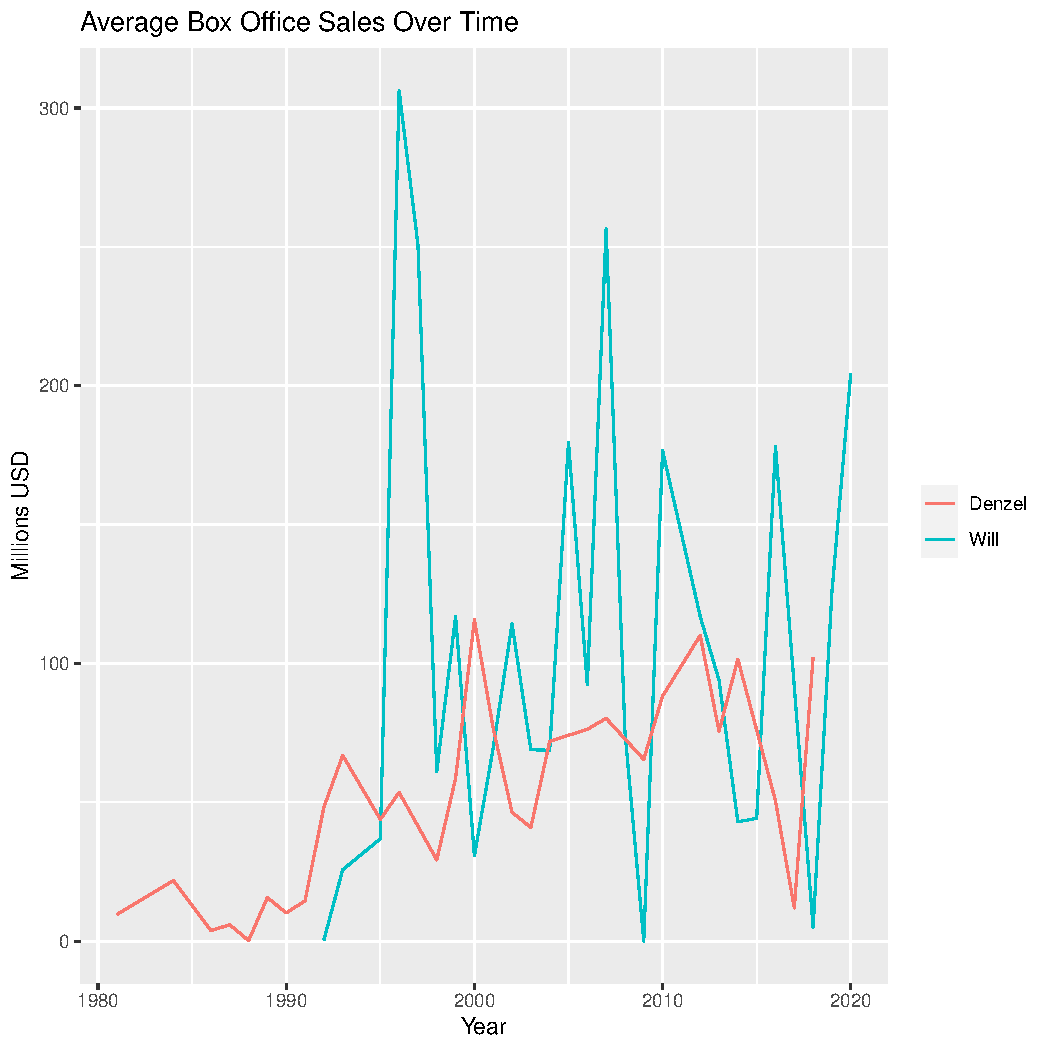
\includegraphics{figures/Blockbuster-Ability.pdf} }
    \end{center}
    \hrule
      \vspace{2mm}
    \caption{ \textbf{Average Movie Revenue Year-by-year:} \newline \footnotesize{ The existence
    of Blockbuster movies can be measured as the volatility of this graph}  }
    \vspace{2mm}
    \hrule
\end{figure}

\begin{figure}[!ht]
 \label{fig:one-graphic}
%% figures have hrule, tables have hline
    \begin{center}
        \scalebox{1.00}{    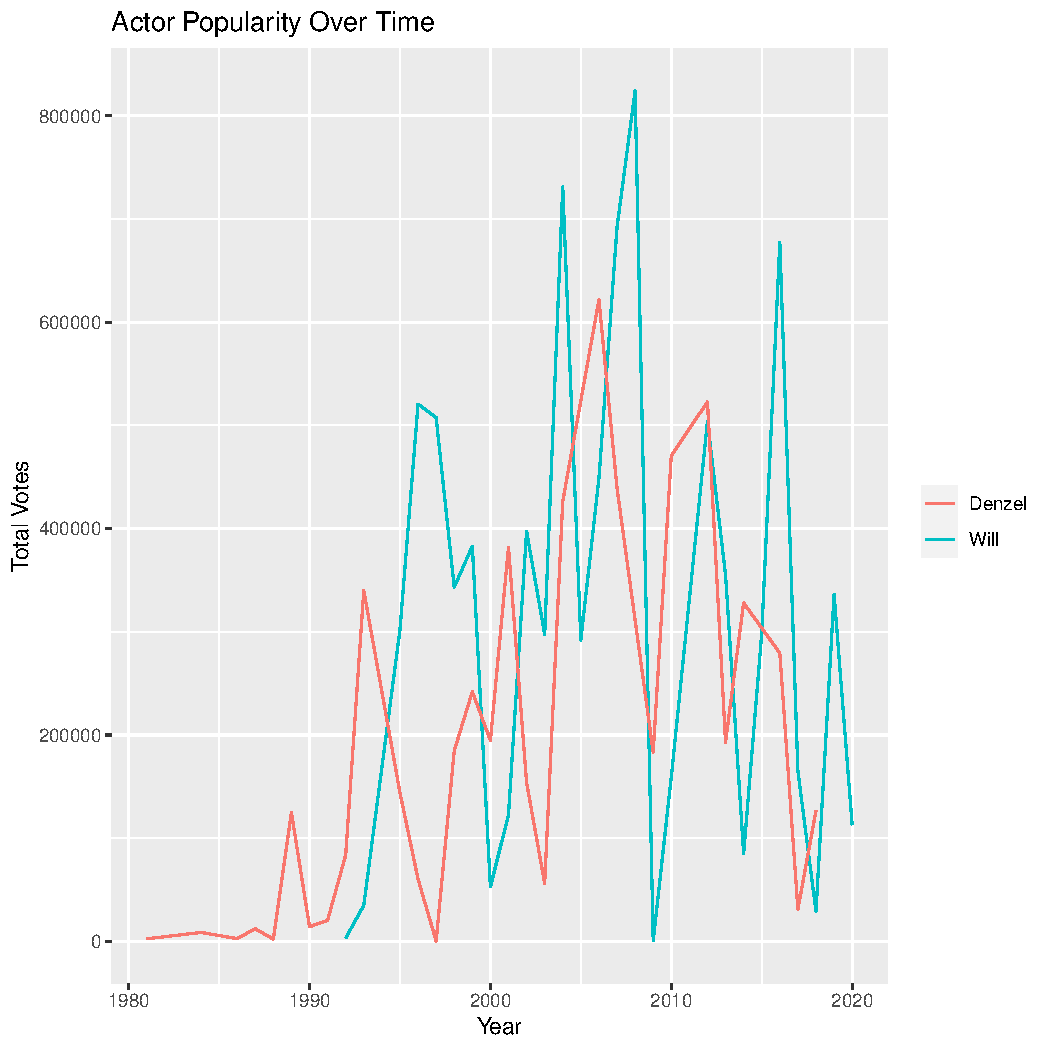
\includegraphics{figures/Pop-Over-Time.pdf} }
    \end{center}
    \hrule
      \vspace{2mm}
    \caption{ \textbf{Actor Popularity Year-by-year:} \newline \footnotesize{ This visual
    can be used to view the public's interest in an actor over time}  }
    \vspace{2mm}
    \hrule
\end{figure}

\section{Conclusion}
\label{sec:conclusion}

The visuals make it clear that Will Smith is consistently able to
``Knock it out of the park'' with his performances at a greater scale
then Denzel Washington. \newline

\noindent The higher peaks on the visual: ``Average Box Office Sales
Over Time'' (Figure 5) indicate that his performances have consistently
brought more revenue on average, and include a greater probability for a
blockbuster movie. This is re-enforced (although not quite as
unmistakably) in the visual ``Actor Popularity Over Time'' (Figure 6)
\newline

\noindent In Conclusion, it is clearly in the best financial interest of
any producer to cast Will Smith rather than Denzel Washington. In every
practical sense, Will Smith is the better actor.




%% appendices go here!


\newpage
\theendnotes

%%%%%%%%%%%%%%%%%%%%%%%%%%%%%%%%%%%  biblio %%%%%%%%
\newpage
\begin{auxmulticols}{1}
\singlespacing 
\bibliography{./../../latex-setup/biblio/master.bib}

%%%%%%%%%%%%%%%%%%%%%%%%%%%%%%%%%%%  biblio %%%%%%%%
\end{auxmulticols}

\newpage
{
\hypersetup{linkcolor=black}
\setcounter{tocdepth}{3}
\tableofcontents
}



\end{document}